\section{Konzept}
Das folgende Kapitel gibt einen Überblick über das Konzept. Es ist gegliedert in die verschiedenen Aspekte der Schaltung.
\subsection{Mechanischer Aufbau}
Der mechanische Aufbau ist durch das Printdesign geprägt. P3T7 besteht aus einem ATmega2560-Board, welches mit 2 «Shields» bestückt wurde. Auf dem obersten Layer befinden sich unter anderem die benötigten Messshunts, der Spannungsteiler, das Netzteil für die $\pm 5V$ Versorgung sowie Sicherungen, welche bei zu hohen Strömen auslösen. Auf dem 2. Layer werden die Messsignale aufbereitet und anschliessend an den Mikrocontroller weitergeben. Das Mikrocontrollerboard ist mit den Massen 54 x 100 der kleinste Layer und wird vom zweiten Print (90 x 125) komplett «verdeckt». Der oberste Print ist um 20 mm seitwärts zum zweiten Layer versetzt und zudem 5 mm schmäler. Durch dies kann durch Distanzbolzen im Gehäuse der Print befestigt werden. Das Gehäuse besitzt eine Kabelverschraubung, durch welche ein SEV 1011 Stecker Typ 12 befestigt ist. Auf der entgegengesetzten Seite können Verbraucher über eine SEV 1011 Steckdose angeschlossen werden.
Das Gehäuse wird durch 4 Schrauben geschlossen. Durch das Kunststoffgehäuse werden jegliche Berührungen mit elektrisch leitenden Teilen verhindert. Falls die Sicherung ansprechen sollte, muss das Gerät vom Netz getrennt werden, bevor die Sicherung ausgewechselt werden kann. 


[Bild ergänzen]

\subsection{Elektrischer Aufbau}
Der elektrische Aufbau gliedert sich in vier verschiedene Teile. Auf dem obersten Print wird mit Netzspannung gearbeitet. Auf dem folgenden Print befindet sich der digital Bereich und der analoge Bereich. Im Digitalbereich ist die Verbindung zu den verschiedenen Bauteilen Realisiert. Es sind eine Realtimelclock, welche folgend nur noch als RTC bezeichnet wird, ein Flashspeicher und ein Bluetooth-Modul vorhanden. Die RTC wird gebraucht, um einen Zeitstempel den Daten beizugeben. Der Flashspeicher wird verwendet um Daten über einen längeren Zeitraum zu speichern und um die Daten nicht nicht-flüchtig zu speichern. Und das Bluetooth Modul wird gebraucht, um eine drahtlose Verbindung zum PC herzustellen. Im analogen Bereich wird die Signalaufbereitung gemacht, welche in einem separaten Kapitel behandelt wird. Die unterste Schicht ist ein Arduino Mega, welcher die Recheneinheit des P3T7 darstellt.

\begin{figure}[H]
\begin{center}
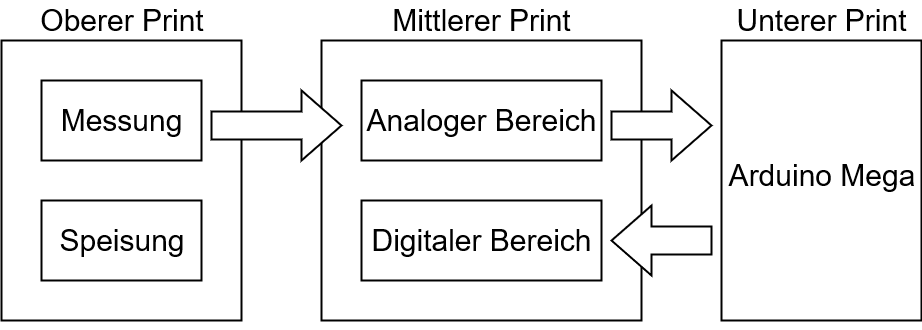
\includegraphics[width=0.9\textwidth]{images/Konzept_Elektrischer_Aufbau.png}
\caption{Konzept Elektrischer Aufbau}
\end{center}
\end{figure}


\subsection{Firmware Aufbau}
Domi neu Schreiben

[ Abbildung folgt noch ]  

\subsection{Software Aufbau}
Die Software stellt die Schnittstelle zwischen dem Menschen und dem P3T7 dar. Sie soll dazu dienen die Daten aus dem P3T7 zu lesen und sie für weitere Berechnungen bereitzustellen. Damit die Daten einfach weiterverarbeitbar sind, kann mithilfe der Software ein CSV-File generiert werden. Dieses kann leicht in Excel oder Matlab importiert werden. Des Weitern werden Berechnungen mit der Software gemacht, für welche der Controller zu schwach ist und um Speicherplatz auf dem P3T7 zu sparen.

\begin{figure}[H]
\begin{center}
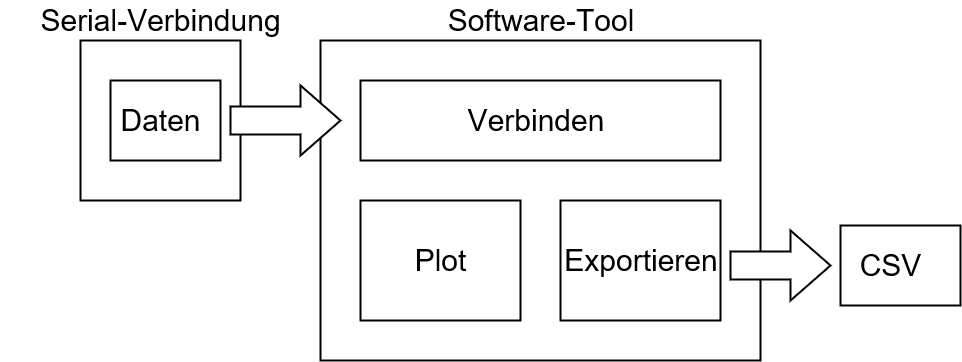
\includegraphics[width=0.9\textwidth]{images/Konzept_Software.png}
\caption{Konzept Software}
\end{center}
\end{figure}

Die Software stellt auch einen Plot mit den ausgelesenen Daten zur Verfügung. Der Plot soll dem User die Möglichkeit geben die Daten zu validieren, bevor er sie weiterverarbeitet. Die Software ist nicht geeignet, um die Daten zu verarbeiten.